% !TEX root = main.tex

\section{Lecture 20: Boundary fluxes and KPP boundary layer scheme}
\begin{flushright}\textbf{[by Fabio Boeira Dias]}\end{flushright}

Ocean General Circulation Models (OGCMs) and coupled ocean-sea ice models are forced at the air--sea boundary by the atmosphere. Widely used by the community, the Coordinated Ocean-sea ice Reference Experiment (CORE, \citeauthor{Griffies2009}, \citeyear{ Griffies2009}) was the first initiative to compile a common protocol to run OGCMs using a common atmospheric forcing based on the fluxes from \cite{Large2004}. The CORE forcing has been used for ocean-sea--ice model intercomparison in several studies (e.g.\ \citeauthor{Danabasoglu2014}, \citeyear{Danabasoglu2014}; \citeauthor{Downes2015}, \citeyear{Downes2015}), but it has not been updated since 2009. To fill this gap, the Japanese Meteorological Agency, in collaboration with the CLIVAR Ocean Model Development Panel, has developed a new product -  the JRA-55-do (driving ocean) \citep{Tsujino2018}, with significant higher horizontal and temporal resolution and planned to be frequently extended to the near present. These atmospheric forcing protocol provides the momentum, heat and hydrological exchanges required to drive the ocean and sea-ice fields. In this lecture, we discuss briefly the boundary fluxes and the boundary layer scheme used in ocean and ocean-sea ice models.\\
%% {\color{Green}In the last decade, the Coordinated Ocean-sea ice Reference Experiment (CORE, \citeauthor{Griffies2009}, \citeyear{ Griffies2009}), based on the fluxes from  has been widely used by the ocean modellers in several studies \citep{Danabasoglu2014, Downes2015}, which is now being slowly replaced by a new product developed by the Japanese Meteorological Agency - the JRA-55-do (Driving Ocean) \citep{Tsujino2018}, which improved horizontal and temporal resolutions and adjustments methods, planned to be update to the near-present frequently.}{\color{red}[This sentence is \textbf{extremely long} and convoluted -- could you rephrase?]} These atmospheric forcing {\color{red}protocol} provides the momentum, heat and hydrological exchanges required to drive the ocean and sea-ice fields. In this lecture, we discuss briefly the boundary fluxes and the boundary layer scheme used in ocean and ocean-sea ice models.\\

\begin{figure}[h!]
  \centering
  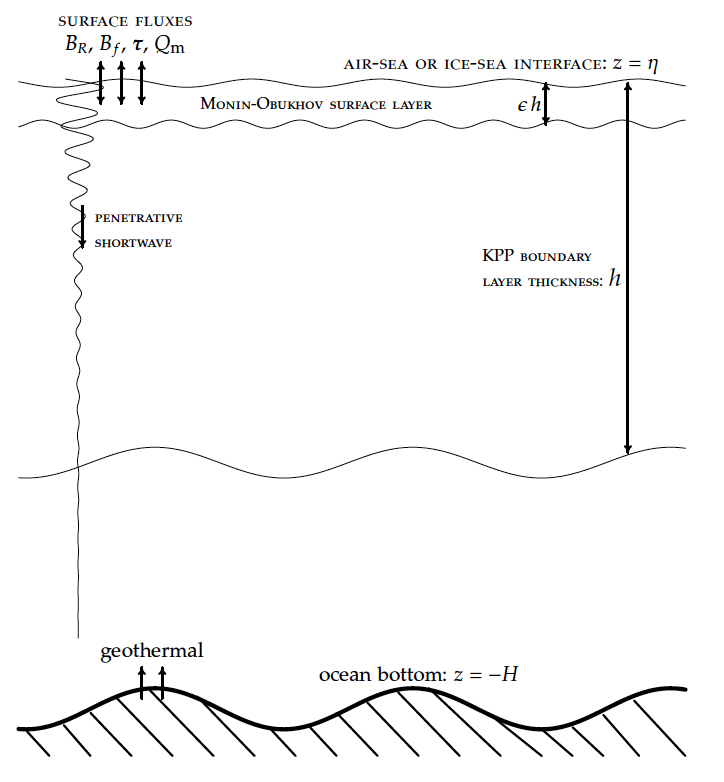
\includegraphics[width=3in]{figures/Figure81_CVmix_manual.png}
  \caption{Figure and caption (modified) from \cite{Griffies2015b}: ``Schematic of the upper ocean boundary layer regions associated with the KPP boundary layer parameterisation. The upper ocean is exposed to non-penetrative air-sea and ice-sea fluxes of momentum, mass $Q_m$, and buoyancy $B_f$. In addition, there is penetrative shortwave radiation, indicated by the exponentially decaying vertical sinusoidal. The Monin-Obukhov surface layer has a thickness 0.1$h$. The surface layer is where turbulence delivers fluxes to the molecular skin layer for transfer to the atmosphere or ice. The surface layer starts from just beneath the surface roughness elements at the upper ocean interface. Since neither these roughness elements, nor the molecular viscous sublayer, are resolved in ocean models, we assume in practice that the Monin-Obukhov surface layer extends to the sea surface at $z(x,y,t)$. The KPP boundary layer includes the surface layer, and it has a thickness $h(x,y,t)$ determined by the KPP parameterisation. The ocean bottom at $z(x,y)$ is rigid and is exposed to geothermal heating.''}% \textcolor{red}{[Navid: is there a typo in the red? $z=(x,y)$? ]}}
\end{figure}

\subsection{Air-sea fluxes}

The total net surface heat flux ($Q_{AS}$) into the ocean results from the interaction of radiative and turbulent fluxes:
\begin{equation}
    Q_{AS} = Q_{S} + Q_{L} +  \boldsymbol{\tau} + E + Q_{E} + Q_{H},
\end{equation}
where the radiative fluxes comprehend the shortwave solar radiation ($Q_{S}$) and net surface longwave solar radiation ($Q_{L}$). The shortwave radiation is computed from the solar insolation $Q_{I}$ incident on the ocean surface subtracted from the portion reflected from the ocean surface:
\begin{equation}
    Q_{S} = Q_{I}(1 - \alpha),
\end{equation}
with $\alpha$ being the albedo, a function of the clouds and usually with a value of 0.065 for the ocean \citep{Payne1972}. The net surface longwave solar is defined by:
\begin{equation}
    Q_{L} = Q_{A} - \sigma_{\text{SB}} , \mathrm{SST}_{\text{skin}}^{4},
\end{equation}

where $Q_{A}$ is the downwelling longwave flux from the atmosphere, $\sigma_{\text{SB}} = 5.67\times10^{-8}\,\text{W}\,\text{m}^{-2}\,\text{K}^{-4}$ is the Stefan-Boltzmann constant.

The turbulent fluxes include contribution from both latent and sensible heat exchange, which includes the wind stress ($\tau$), %[Navid: I don't understand what this means]
evaporation ($E$), latent heat ($Q_{E}$) and sensible heating ($Q_{H}$), defined by:
\begin{align}
    \boldsymbol{\tau} &= \rho C_{D} \left( \zeta_{10} \right) |\Delta \boldsymbol{U}| \Delta \boldsymbol{U}, \\
    E &= \rho C_{E} \left( \zeta_{10} \right) | q - q_{s} \left( SST \right)| |\Delta \boldsymbol{U}|, \\
    Q_{E} &= \Lambda_{V} E, \\
    Q_{H_{sens}} &= \rho c_{p} C_{H} \left( \zeta_{10} \right) \left( \Theta - SST \right) |\Delta \boldsymbol{U}|.
\end{align}
%{\color{red}[Navid: 1. Ιs there a typo in eq. (20.5)? There are three $|$.\\ 2. Why is $\tau$ bold in eq. (20.4) but not in eq. (20.1)? Is there a typo?]}

These fluxes are parameterised using the Bulk formulae \citep{Large2008} from the near surface atmospheric state (meridional and zonal components of the wind $\boldsymbol{U}$, potential temperature $\Theta$, specific humidity $q$ and density $\rho$) %[Navid: what are all these? Are these introduced to be used in eqs. (20.4-20.7)? If so, you should defined them after those eqs.] 
and the surface ocean state (SST and surface ocean currents). While CORE and JRA-55-do provided the atmospheric state, the ocean state are usually taken from the surface ocean model grid cell. At the time of the CORE bulk formulae was developed, it was considered an ocean model upper-layer of around 10~$m$; as the use of models with higher resolution become more common, a change in the bulk formulae might be required.
%{\color{Green}While CORE and JRA-55-do provided the atmospheric state, the ocean state are usually taken from the surface ocean model grid cell, which is an appropriated choice since the Bulk formulae was developed for the upper-ocean (around 10~$m$ for climate models, which have to be take in account when running a model with higher vertical resolution). \textcolor{red}{[Navid: Again a long sentence that confused me.]}} The turbulent fluxes are defined by:

The dimensionless atmospheric stability ($\zeta_{10}$) uses a reference height of 10~$m$, the specific heat capacity of air is given by $c_{p} \approx 1000.5 \text{J}\,\text{kg}$, $\Lambda_{V} = 2.5 \times 10^{6} \text{J}\,\text{kg}$ is the latent heat of vaporisation for water and the difference between the atmospheric winds and ocean currents is defined by $\Delta \boldsymbol{U} = \boldsymbol{U} - \boldsymbol{U}_{0}$ \citep{Pacanowski1987}.

The methodology for shifting the neutral 10~$m$ transfer coefficients for drag ($C_{D}$), sensible heat exchange ($(C_{h}$) and evaporation ($C_{E}$) are defined in \cite{Large2004}. Following the CORE-I study in \cite{Griffies2009}, most of the ocean is cooled by negative $Q_{H}$ and $Q_{E}$, which makes $\zeta_{10}$ negative and the atmosphere unstable. The majority of models in the \cite{Griffies2009} study computed incorrect transfer coefficients and have a fractional error associated, which is usually greater than unity and larger in regions where high SST and low winds speeds are combined to make a significantly unstable atmosphere. In addition, where these regions experienced significant surface cooling through latent heat flux there are an intensification of the error due to the loss, which makes the heat flux error larger.

\subsection{Boundary layer scheme}

In the 1-dimensional vertical scheme, the time-evolution of a tracer $\bar{\Lambda}$ is:
\begin{equation}
    \frac{\partial \bar{\Lambda}}{\partial t} = \frac{\partial(\overline{w \lambda})}{\partial z} - \frac{\partial \overline{w' \lambda '}}{\partial z},
\end{equation}

where the first term in RHS represents the resolved advection and the second term is the turbulent (subgridscale) correlation. {\color{red}[Navid: What's the overline?]}. {\color{red}The subscrid scale turbulent fluxes need} to be parameterised:
\begin{equation}
    \overline{w' \lambda '} = \overline{w \lambda}^{\text{local}} + \overline{w \lambda}^{\text{non-local}}.
\end{equation}

The turbulent correlation is parameterised as a the local and a  non-local term. The local term is the familiar downgradient diffusion:
\begin{equation}
     \overline{w \lambda}^{\text{local}} = -K \frac{\partial \bar{\Lambda}}{\partial z},
\end{equation}
with $K$ the turbulent diffusion coefficient. The non-local term is given by:
\begin{equation}
    \overline{w \lambda}^{\text{non-local}} = K^{\text{non-local}} \, \gamma,
\end{equation}
where $\gamma$ is the non-local term, which comes from a remotely place in the vertical. An example of the non-local effect is under a negative surface buoyancy forcing, which triggers instabilities that will propagate downward in the ocean boundary layer. The $K^{\text{non-local}}$ is function of a turbulent velocity scale $w$ and a structure function $G$, both only function of the depth $z$:
\begin{equation}
    K^{\text{non-local}} = h \, w(z) \, G(z).
\end{equation}

The depth of the boundary layer is often defined in function of the Bulk Richardson number:
\begin{equation}
    Ri(d) = \frac{(d-d_{r}) \left[ B_{r} - B(d) \right]}{| \boldsymbol{U}_{r} - \boldsymbol{U}(d) |^{2}} + U^{2}_{z},
\end{equation}
where $\boldsymbol{U}(d)$ is the horizontal velocity and $B(d)$ buoyancy at depth $d$ and $B_{r}$ and $\boldsymbol{U}_{r}$ within the Monin-Obukhov surface layer (see Fig \ref{cvmix_fig8.1}). The Richardson critical number ($Ri_{crit}$) is usually defined between 0.25 and 0.3 - which is a tuning parameter of ocean models. Then we can define:
\begin{align*}
    Ri(d) < Ri_{crit} \textrm{ if is within the boundary layer;}\\
    Ri(d) > Ri_{crit} \textrm{ if is outside the boundary layer.}
\end{align*}